% Author        : PokMan Ho pok.ho19@imperial.ac.uk
% Script        : m_ebc7_comparison.tex
% Desc          : model comparison between 2010 and this
% Input         : none
% Output        : pdf comparison report here
% Arguments     : 0
% Date          : Mar 2020

\documentclass[a4paper,11pt]{article}
\usepackage[margin=2cm]{geometry}
\usepackage{graphicx, hyperref, longtable, amsmath, amssymb, csquotes,float,multicol}
\graphicspath{{graph/}{graph/}}
\hypersetup{
	colorlinks=true,
	linkcolor=blue,
	filecolor=blue,      
	urlcolor=blue,
	citecolor=blue
}

\begin{document}
Latest version of ecosystem carbon cycle \href{https://www.sciencedirect.com/science/article/pii/B9780123850058000071}{model}

\begin{figure}[H]
    \centering
    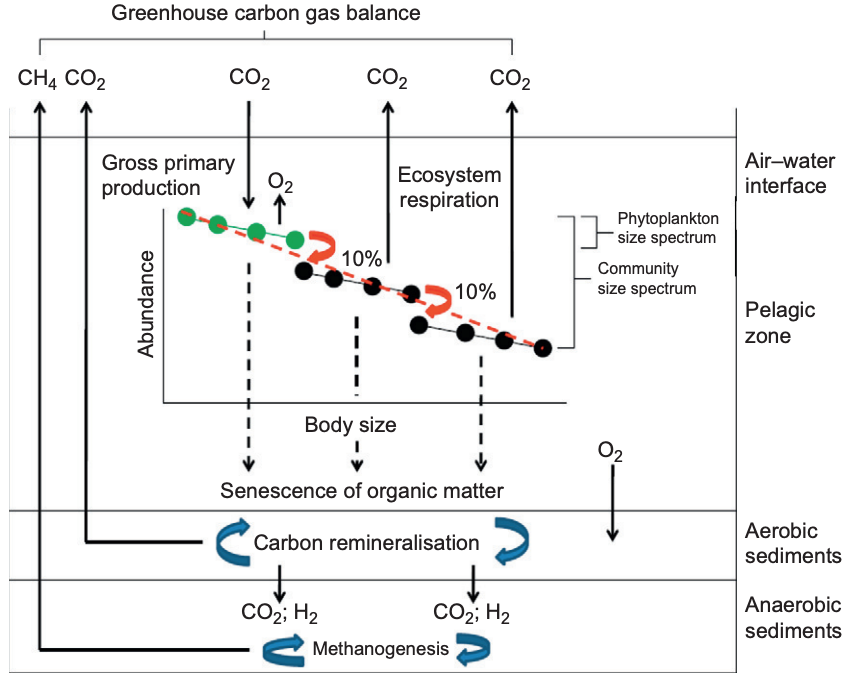
\includegraphics[width=.4\linewidth]{sandbox/graph/paper2010.png}
    \caption{Figure extracted from the 2010 paper, demonstration purpose only}
    \label{ppr10}
\end{figure}

\begin{align}
    GPP &= p_0e^{E_p/kT}M_{TOT}^p\langle M^{1-\alpha}\rangle_p\\
    NPP &= \varepsilon GPP\\
    AR &= (1-\varepsilon)GPP\\
    HR &= r_0e^{E_r/kT}M_{TOT}^r\langle M^{1-\alpha}\rangle_r\\
    ER &= AR + HR\\
    MP &= m_0e^{E_m/kT}M_{TOT}^m\langle M^{1-\alpha}\rangle_m\\
    ER/GPP &= \dfrac{r_0e^{E_r/kT}M_{TOT}^r\langle M^{1-\alpha}\rangle_r}{p_0e^{E_p/kT}M_{TOT}^p\langle M^{1-\alpha}\rangle_p}\text{, which assume AR = 0}
\end{align}

adapted model

\begin{figure}[H]
    \centering
    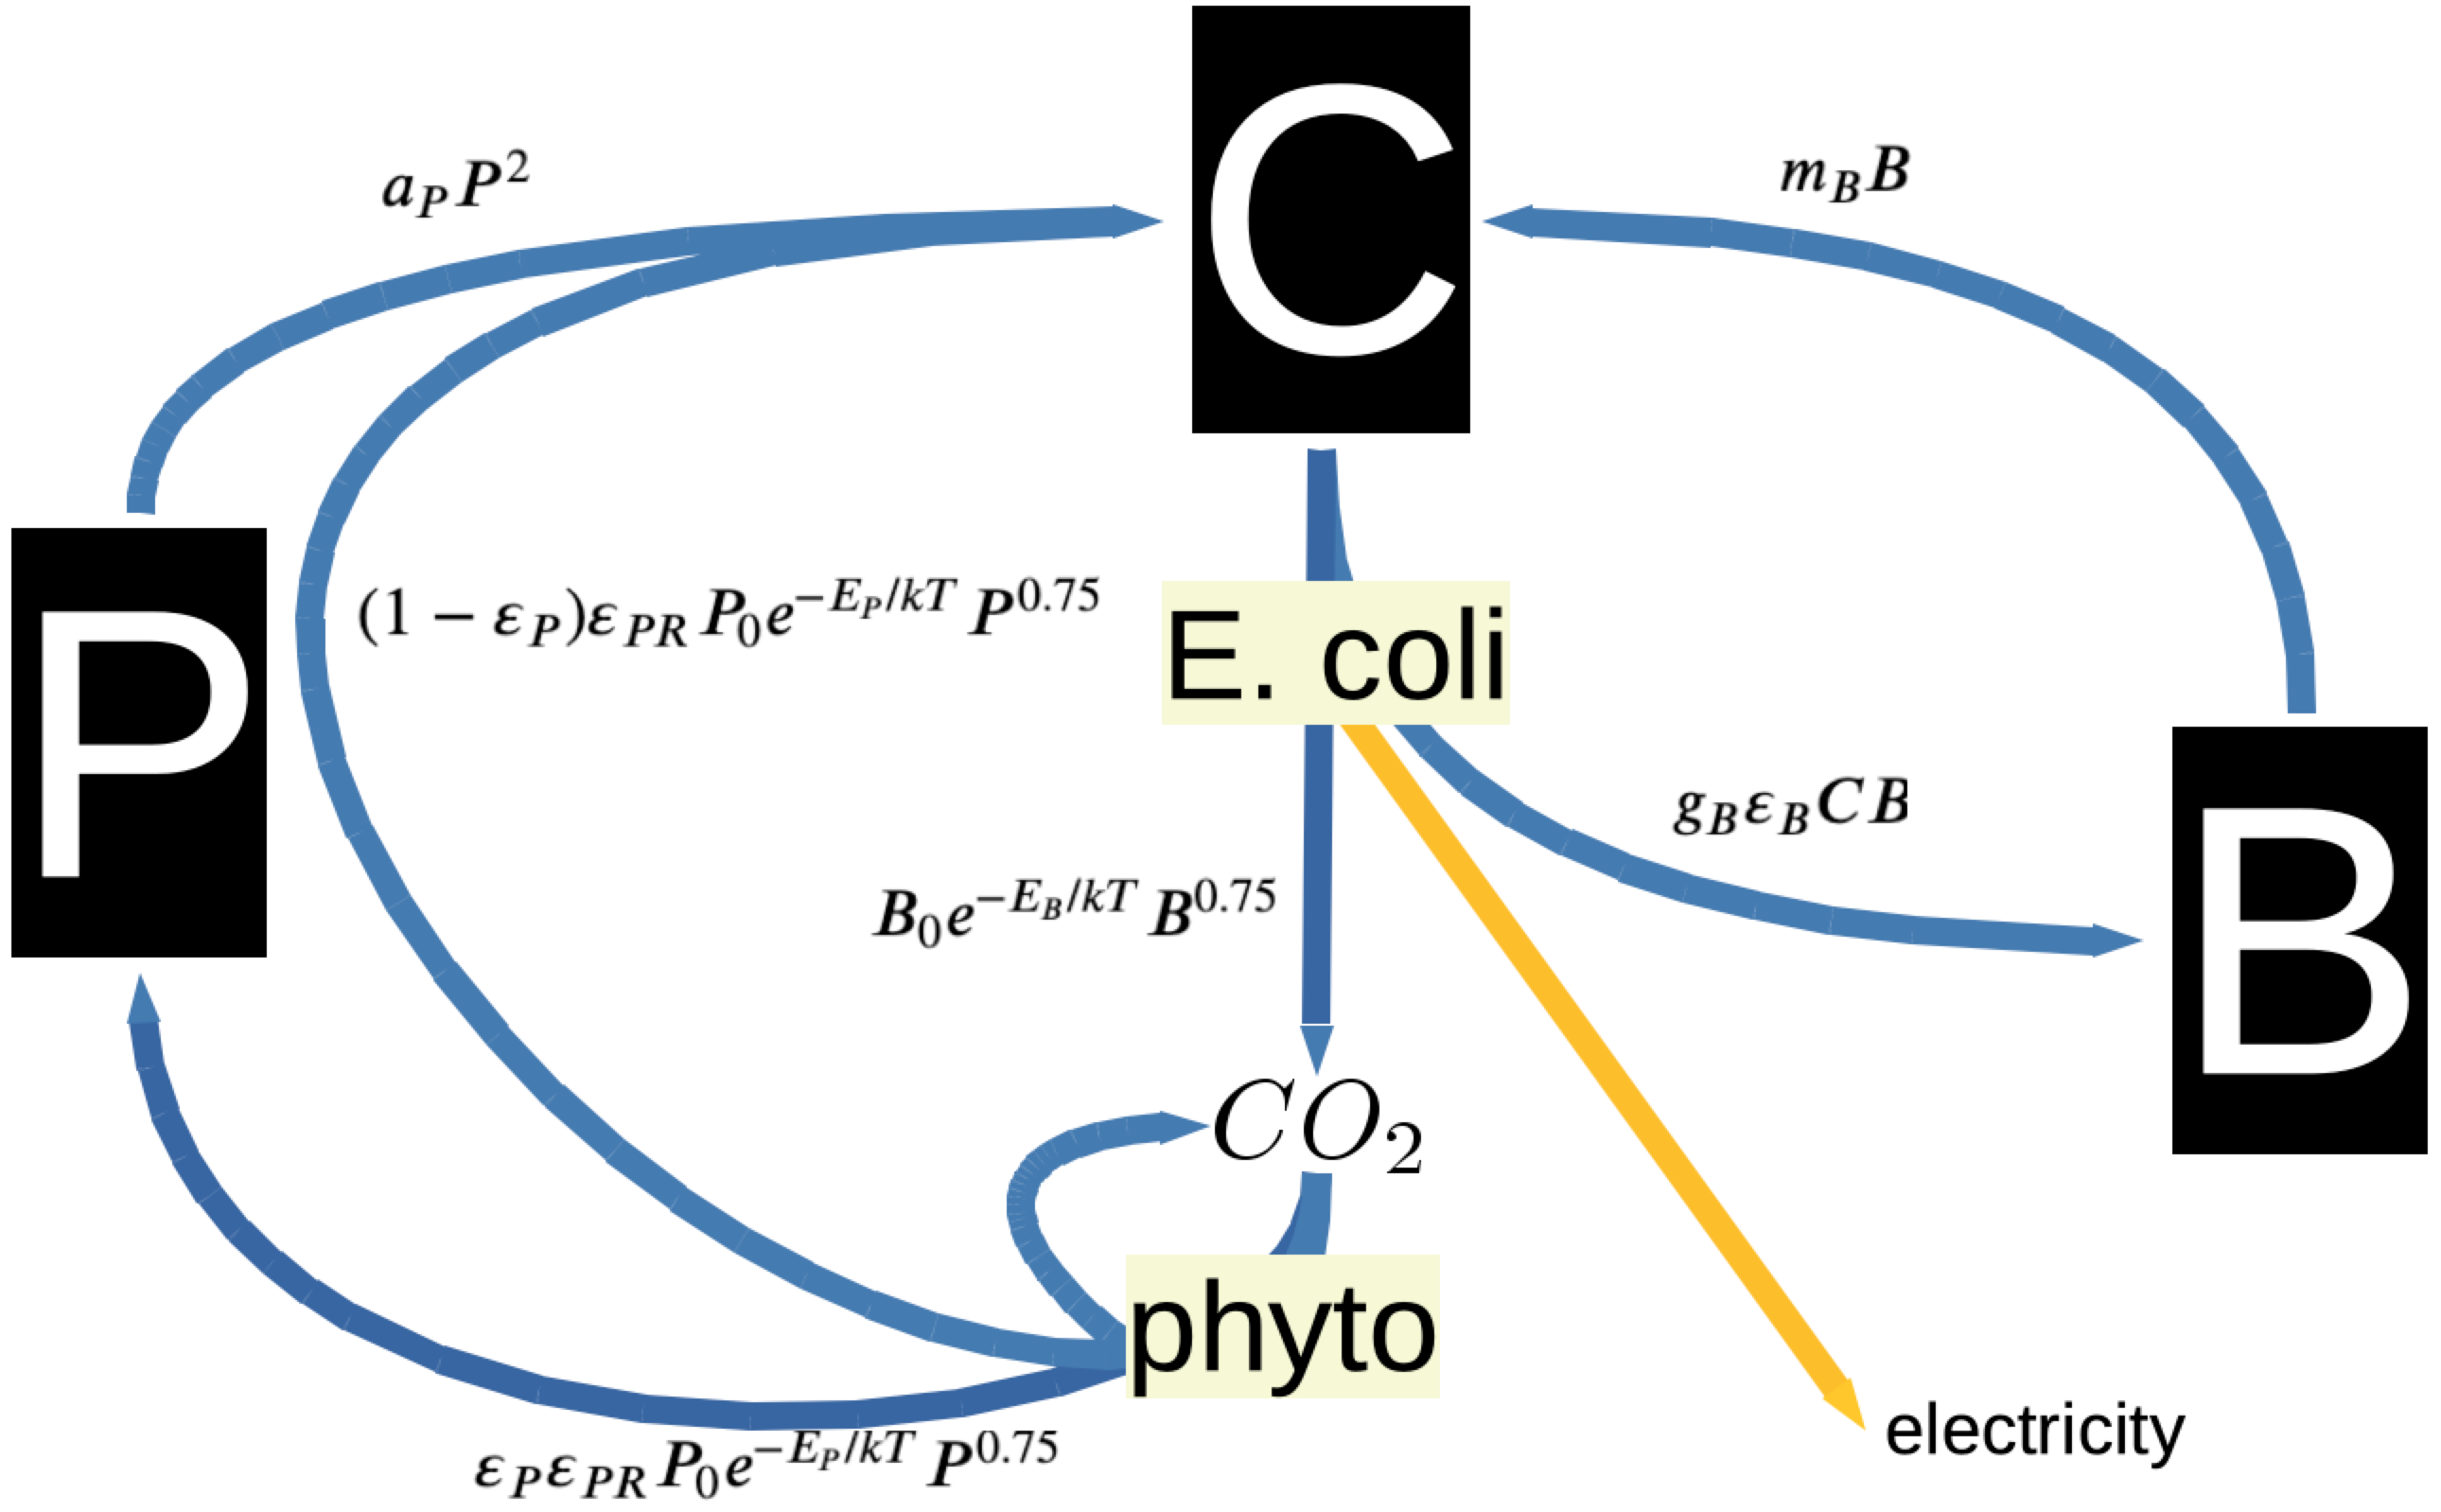
\includegraphics[width=.4\linewidth]{sandbox/graph/ebc7.png}
    \caption{Visualization of solar bio-panel idealized ecosystem}
    \label{ebc7}
\end{figure}

\begin{equation}\left\{\begin{array}{rl}
C'(t) &= (1-\varepsilon_P)\varepsilon_{PR}P_0e^{-E_P/kT}P^{0.75} +a_PP^2 -B_0e^{-E_B/kT}B^{0.75} -g_B\varepsilon_{B}CB +m_BB\\
P'(t) &= \varepsilon_P\varepsilon_{PR}P_0e^{-E_P/kT}P^{0.75} -a_PP^2\\
B'(t) &= g_B\varepsilon_{B}CB -m_BB
\end{array}\right.\end{equation}

problem: photosynthesis \& respiration term is extremely small, much much smaller than the intraspecific interference term

\clearpage

\begin{longtable}{p{.15\linewidth}|p{.35\linewidth}|p{.35\linewidth}|}
& 2010 & CPB model\\\hline
similarities & \multicolumn{2}{p{.7\linewidth}|}{\begin{itemize}
    \item use of Arrhenius equation: from the energy exchange aspect
    \item carbon balance as system indicator of stability
\end{itemize}}\\\hline
differences & \begin{itemize}
    \item phytoplankton, heterotroph, methanogens
    \item aims at model the efflux of greenhouse gases (GHG) to atmosphere under warming situation
    \item calculation based upon stabilized ecosystem
    \item assume every organism under consideration has different metabolic rate / body sizes
    \item focus on carbon balance based on photosynthesis-respiration balance
    \item biomass in the view of cellular organism individuals
\end{itemize} & \begin{itemize}
    \item phytoplankton, detritivore (heterotrophic specialist), organic matter
    \item aims at model system carbon sequestration and electricity generation ability from establishment to possible equilibria
    \item forward simulate ecosystem interaction evolution
    \item single species pair setting, assume every individual from the same functional lineage is identical in size
    \item focus on carbon balance based on organism biomass pool flux and biomass accumulation
    \item biomass in the view of lineage / population
\end{itemize}
\end{longtable}

\end{document}